%!TEX root = main.tex

\section{Introduction}
\label{sec:intro}

This paper proposes a novel solution to recommend travel routes in cities. 
Large amount of location traces is becoming available from the ubiquitous location tracking devices. 
For example, FourSquare, the local search and discovery service has 50 million monthly users who have made 8 billion check-ins~\cite{4sq}; Flickr, the online photo-sharing site, hosts over 2 billion geo-tagged public photos~\cite{flickr}. Such large-amounts of travel data provides new opportunities for better 
travelling planning traditionally done with written travel guides, 
choosing and ranking locations for a variety of activities from dining to recreation, 
and potential new solutions to orienteering and routing problems. 
Good solutions to these problems will in turn lead to better urban experiences for residents and visitors alike, and foster sharing of even more location-based behaviour data. 
\eat{
Location based information sharing services provided by online social media,
for example Facebook, Twitter and Flickr, generate data with geographical information,
together with time-stamps and user tags.
This enables us to identify the trajectory of a particular user as he or she travels through
a city. By combining trajectories of multiple users in a particular city, we
have an opportunity to explore patterns of tours. Using POI properties such as the type
or category of the site visited,
as well as transition patterns between different POIs,
we obtain a way to recommend high quality trajectories to travellers.
}

There are few common settings of recommendation problems for locations and routes, as illustrated in Figure~\ref{fig:threesettings}. 
The first setting can be called points-of-interest (POI) recommendation (Figure~\ref{fig:threesettings}(a)), here each location (e.g. A to E) is scored with geographic property and behavioural information such as category, reviews, popularity, spatial information such as distance and travel time uncertainty, and temporal information such as time of the day or day of the week.  There is a rich collection of recent literature on this problem~\cite{bao2015recommendations,yin2015joint,shi2011personalized,lian2014geomf,liu2014exploiting,yuan2013timeaware,hsieh2014mining,gao2013temporal,yuan2014graph}, including recent surveys~\cite{bao2015recommendations,zheng2014urban}. 
Figure~\ref{fig:threesettings}(b) illustrates the problem of next location recommendation\cite{ijcai13,aaai16,baraglia2013learnext,zhang2015location}, here the input is a partial trajectory (e.g. started at point A and currently at point B), the task of the algorithm is to score the next candidate location (e.g, C, D and E) based on the perceived POI score and transition compatibility with input $A\rightarrow B$. 
    The last setting is route recommendation, as illustrated in Figure~\ref{fig:threesettings}(c). Here the input are some deciding factors about the desired route, e.g. starting point A and end point C, along with auxiliary information such as the desired length of trip. The algorithm needs to take into account location desirability (as indicated by node size) and transition compatibility (as indicated by edge width), and compare route hypotheses such as A-D-B-C and A-E-D-C. Existing work in this area either uses heuristic combinations of location and routes~\cite{ijcai15,lu2012personalized}, or formulates an optimisation problem that were not informed or evaluated by behaviour history~\cite{gioniswsdm14,chen2015tripplanner}. Joint learning of locations preferences and routes remains an open problem.

\begin{figure*}[t]
	\centering
	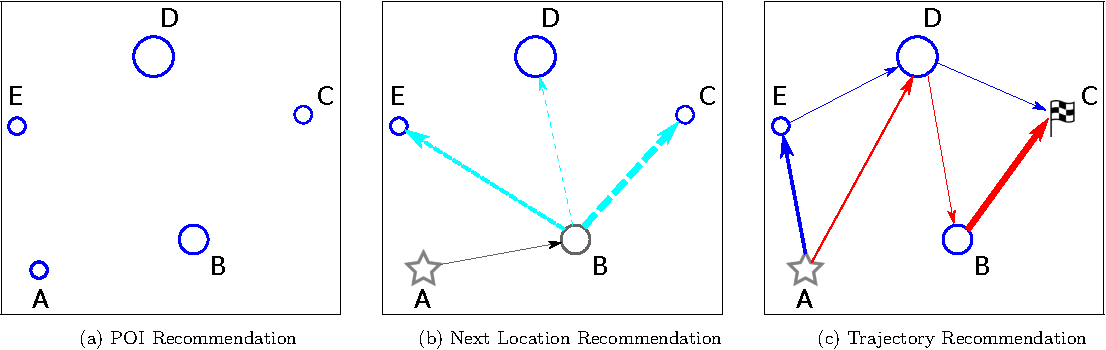
\includegraphics[width=\textwidth]{fig/fig1-flavours.pdf}
	\caption{Three settings of trajectory recommendation problems: (a) POI recommendation, (b) next location recommendation, and (c) trajectory recommendation. Node size: POI score; edge width: transition score between pairs of POIs; grey: input query; star: starting location; flag: ending location. See the 2nd paragraph of Section~\ref{sec:intro} for details.
}
	\label{fig:threesettings}
\end{figure*}

We propose a novel way to learn point and route preferences jointly. 
Our solution consist of several main parts. 
We propose a learning to rank formulation to capture the preference of POIs given the starting and ending points of a trajectory. We model pair-wise transition patterns between POIs by factorising the transition likelihoods along five different types of location properties, % of the Markov chain between POIs
this alleviates data sparsity between each pair of POIs and allows POIs of the same type and neighborhood to share parameters.
We combine the results of point and transition ranking using inference in a Markov chain and route planning techniques. We further propose a novel way to jointly learn point and transition scores with Structured Support Vector Machine (StructuredSVM). We evaluated the proposed algorithm on photo trajectories in five different cities, with a traditional metric $F_1$ on POIs as well as a new pairs-$F_1$ metric specifically designed for trajectories. We found that the learning-based approaches generally out-perform heuristic route recommendation~\cite{ijcai15}. Incorporating transition into point ranking improves the pairs-$F_1$ metric for the correct sequencing of POIs, and that routing algorithms that disallow sub-tours generally out-perform Markov chain methods. 

\eat{and evaluate the quality of POIs in recommended trajectories in terms of trajectory F$_1$-score~\cite{ijcai15}. One problem with the F$_1$-score on POIs is that it ignores
the order in which sites are visited.
We propose a new performance measure by applying F$_1$-score on pairs of POIs.
Experimental results on five trajectory datasets show performance improvements over the state-of-the-art methods and
reveal many interesting properties of trajectories in different datasets.
}

The main contribution of this work is as follows: 
\begin{itemize}
\setlength{\itemsep}{-2pt}
\item We propose a novel algorithm to jointly optimise point preference and route plan.
\item Our approach is feature-driven and learns from past behaviour without having to design specialised treatment for spatial, temporal and social information. It currently incorporates information about location, POI categories and behaviour history, and can use additional social or time information as long as they are  encoded in features. 
\item We have shown strong performances compared to recent results~\cite{ijcai15}, we also quantify the contribution from the different components, such as point ranking, scoring transitions, and routing. 
\item We propose a new metric to evaluate trajectories: pairs-$F_1$, which has the property of being between 0 and 1, and being 1 if and only if two trajectories are exactly the same. Our benchmark data and results are publicly available.
\end{itemize}
